\section{A polynomial approximation for expected depth}
\label{sec:mass-improvement}

We give one algorithm for arbitrary positive rational priors. The
prior is fixed throughout the construction: a query's expected cost
is the mass of hypotheses that reach it. At a state admitting a
balanced supplied line, the algorithm queries that line. At a flat
state, it tests hull blocks until a positive answer is found or a
full negative cover identifies the zero-pattern singleton. After a
positive answer it learns the complete hull pattern and recurses
within that pattern class. Its polynomial-time factor is below
$5.182976$.

Two costs need to be controlled at a flat state: finding a positive
block and recovering the rest of its pattern. The useful comparison
is an entire pattern stage. Queries that become constant after the
pattern class is known provide credit for discovery. Information
already learned during discovery reduces the entropy still needed
for endpoint recovery. Charging the stage to these two decreases
lets us sum the bound over the recursive tree. The geometric and
interval-coverage primitives were proved in
Sections~\ref{sec:geometry} and~\ref{sec:scheduling}.

\subsection{The algorithm and its supporting propositions}

Use fixed calibration parameters $\beta,\delta,p_*$, whose values are
deferred to Section~\ref{sec:two-phase}. Here
$3<\beta<4$, $0<\delta<1/3$, and $0<p_*<1/2$.
A line is mass-balanced if each side has mass at least $\delta w(S)$.
Otherwise the common-witness construction supplies the normalized hull.
Keep its full cyclic order, including the constant-negative origin
marker when it is a hull vertex. Candidate blocks are its edges: each
block uses only its one or two real supplied endpoint tests.

Write $\Pi$ for the full-pattern partition and $A_0$ for its
all-negative class, which is empty or a singleton. Throughout this
section the prior weights retain their original normalization:
\[
 w=w(S),\qquad p_0=w(A_0),\qquad b=w-p_0,\qquad
 I=I(S,\Pi),\qquad \Delta=\Delta_{\mathrm E}(S,\Pi).
\]
The quantity $I$ is the information needed to learn the pattern;
$\Delta$ is the optimal cost made unnecessary after its class is known.
These are comparison quantities used in the analysis; the algorithm
chooses its schedule from observable pattern masses and coverage scores.

\paragraph{Choose the coverage schedule.}
Small budgets locate common positive patterns quickly; larger
budgets eventually cover every positive pattern. Exact budgeted
coverage chooses the blocks, while greedy ordering places their
largest new masses first. We vary the first two budgets because
these early decisions have the greatest effect on expected cost.
Compute a maximum-weight block cover $Q_k$ for each budget
$k<k_{\min}$ and a minimum full cover $Q_*$ of size $k_{\min}$.
To justify these DPs, Lemma~\ref{lem:hull-structure} gives each
positive pattern one circular vertex interval. The hull edges
incident to that interval form one circular interval in the edge
order, so Lemmas~\ref{lem:minimum-interval-cover}
and~\ref{lem:budget-coverage} apply to the block demands.
For a geometric shift $u$, set
$k_j=\lfloor\beta^ju\rfloor$. Try the following initial
budget sequences, followed by the common geometric tail:
\[
 \begin{array}{ll}
 q,r,k_2,k_3,\ldots,
 &1\le q\le6,\quad r\in\{k_1-1,k_1,k_1+1\},\quad q<r<k_2,\\
 q,k_2,k_3,\ldots,&1\le q\le6.
 \end{array}
\]
At each budget $k<k_{\min}$, greedily append productive unused
blocks of $Q_k$, ordering them by newly covered weight. At the first
budget reaching $k_{\min}$, use $Q_*$ and finish. There are at most
twenty-four variants per shift.

Refine the usual geometric shift partition by the constant set
\begin{equation}\label{eq:initial-shift-refinement}
 \frac{k}{\beta},\ \frac{k}{\beta^2}\in[1,\beta),
 \qquad 1\le k\le\lceil\beta^3\rceil.
\end{equation}
Represent each open cell by any point in it, and also include each
left breakpoint. Thus initial budgets remain represented even when
$k_{\min}$ truncates the ordinary geometric partition. In particular,
$r=k_1-1$ can first complete the cover at $k_1=k_{\min}+1$.

\paragraph{Choose the two-endpoint mode.}
Finding a positive block leaves a choice: stop at its first positive
endpoint, or ask the other endpoint as well. The extra answer can
save later decoding cost, so comparing only the number of discovery
queries would miss its benefit. The following score includes both
the immediate query saving and a guaranteed information credit.
On an all-negative schedule prefix, let $x\le y$ be the newly hit
masses exclusive to the two endpoints of the next block, and let
$z$ be their shared mass. Put $h_*=1-2p_*$ and define the rational
entropy credit and saving
\begin{equation}\label{eq:rational-block-saving}
 \begin{aligned}
 E_*(a,z)&=\min\{(h_*/p_*)a,\ h_*(a+z),\ (h_*/p_*)z\},\\
 D(x,y,z)&=\max\{y,\ x+y-z+E_*(y,z)\}.
 \end{aligned}
\end{equation}
The first choice stops at the first positive answer, asking the
smaller exclusive mass first. The second choice asks both endpoints,
asking the larger exclusive mass first. The latter order gives at
least as much credited information because each of the three affine
terms defining $E_*(a,z)$ is nondecreasing in $a$, and so is their
pointwise minimum. Choose the endpoint with the larger saving.
The exact binary-entropy bound behind $E_*$ is checked
only in the final calibration.

For a candidate schedule $G$, let $k_A$ be its first block hitting
positive class $A$, and set
\begin{equation}\label{eq:adaptive-shift-objective}
 F_*(G)=2\sum_{A\ne A_0}w(A)k_A+2p_0|G|
             -\sum_{\text{blocks}}D.
\end{equation}
This one score prices positive discovery, the entire zero-pattern
waiting route, and the mode savings. Choose its minimum. At each
positive exit, build the legal expected-cost endpoint decoder and
attach the recursive tree for its full pattern class.

\begin{algorithm}[H]
\caption{Rational choice between stopping and querying both endpoints}
\label{alg:block-mode}
\KwIn{New exclusive masses $x,y$, shared mass $z$;
calibrated $p_*$ and $h_*=1-2p_*$.}
\KwOut{Stored endpoint order, mode, and rational saving $D$.}
Label the endpoints so $x\le y$\;
$E\gets\min\{(h_*/p_*)y,\ h_*(y+z),\ (h_*/p_*)z\}$\;
\eIf{$y\ge x+y-z+E$}{
 Record stop mode with the $x$ endpoint first; $D\gets y$\;
}{
 Record query-both mode with the $y$ endpoint first;
 $D\gets x+y-z+E$\;
}
\KwRet the recorded order, mode, and $D$\;
\end{algorithm}

These new masses are computed on the all-negative prefix before the
block. In the stored discovery stage, stop mode ends at the first
positive answer; query-both mode learns both bits before endpoint
recovery. Their union and first-cover rank are the same.


\begin{algorithm}[H]
\caption{\ExpectedTree: the polynomial expected-depth algorithm}
\label{alg:expected-tree}
\KwIn{State $S$, original positive rational priors;
calibrated $\beta,\delta,p_*$.}
\KwOut{A supplied-query identification tree.}
\If{$|S|\le1$}{\KwRet its leaf\;}
\If{a mass-balanced supplied line $\ell$ exists}{
 \KwRet $\ell$ with children $\ExpectedTree(S_\ell^-)$
 and $\ExpectedTree(S_\ell^+)$\;
}
Compute $\HullData(S)$, its pattern classes, and zero weight $p_0=w(A_0)$\;
\eIf{there are at most two real extreme hull tests}{
 Build their direct full-pattern stage\;
}{
 Use edges of the full hull as blocks, retaining its free origin marker\;
 Select the schedule and stored modes by Algorithm~\ref{alg:two-phase-family}\;
 Build discovery along its all-negative prefix, with those modes on each first hit\;
 At each positive exit build expected $\EndpointCode$ to recover the full pattern\;
}
Attach $\ExpectedTree(A)$ to each nonzero pattern class $A$\;
Use a zero-query leaf for the zero singleton; omit it when absent\;
\KwRet the tree after contracting constant and cached questions\;
\end{algorithm}

The cases in the algorithm have a direct purpose: singleton states
already identify their hypothesis, balanced lines split immediately,
and flat states use the hull schedule to discover a full pattern before
recursing within its class. Each recursive call reuses the fixed
calibration and full supplied-query family. Since the incidence table
and prior weights are known, schedule scores, endpoint modes, and child
codes can all be determined before the hidden hypothesis is queried;
the routine therefore returns a concrete tree for it to follow.


\begin{algorithm}[H]
\caption{Two-budget schedule selection for \ExpectedTree}
\label{alg:two-phase-family}
\KwIn{Positive-pattern block demands, original weights, zero weight $p_0$;
calibrated $\beta,p_*$.}
\KwOut{A schedule and stored modes minimizing the rational score $F_*$.}
Compute $Q_*$ of size $k_{\min}$ and every $Q_k$ for $k<k_{\min}$\;
Refine the geometric shift cells by \eqref{eq:initial-shift-refinement}\;
\ForEach{breakpoint or one interior representative $u\in[1,\beta)$}{
 $k_1\gets\lfloor\beta u\rfloor$; $k_2\gets\lfloor\beta^2u\rfloor$\;
 \For{$q=1,\ldots,6$}{
  $\mathcal V\gets\{(q,0)\}\cup
   \{(q,r):r\in\{k_1-1,k_1,k_1+1\},\ q<r<k_2\}$\;
  \ForEach{$(q,r)\in\mathcal V$}{
   $G\gets$ empty order\;
   Process $q$, then $r$ if $r>0$, then $k_2,k_3,\ldots$\;
   At each budget $k$, greedily append productive unused blocks
   from $Q_k$ if $k<k_{\min}$, and from $Q_*$ otherwise\;
   Stop these phases at the first budget reaching $k_{\min}$\;
   Compute the new masses and stored mode of each block by
   Algorithm~\ref{alg:block-mode}\;
   Retain $(G,\text{modes})$ with its rational score $F_*(G)$\;
  }
 }
}
\KwRet a retained pair of minimum score\;
\end{algorithm}

\begin{figure}[htbp]
\centering
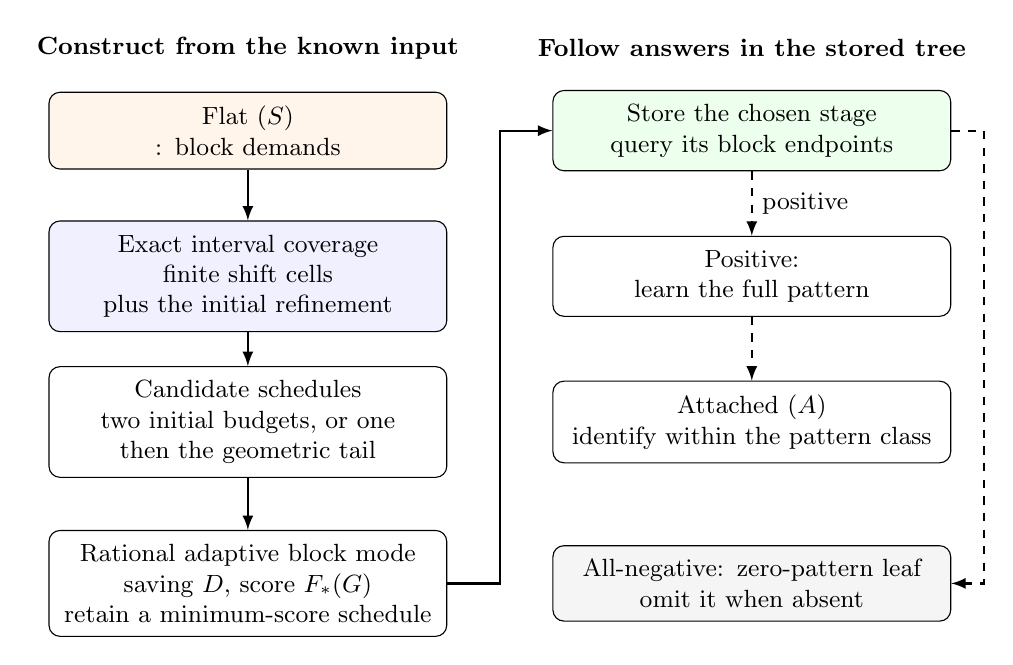
\begin{tikzpicture}[every node/.style={font=\small},
  box/.style={draw,rounded corners,align=center,inner sep=5pt,text width=4.7cm},
  arr/.style={-latex,thick},exec/.style={-latex,thick,dashed}]
  \node[font=\small\bfseries] at (-3.2,1.05) {Construct from the known input};
  \node[font=\small\bfseries] at (3.2,1.05) {Follow answers in the stored tree};
  \node[box,fill=orange!8] (hull) at (-3.2,0)
    {Flat \ExpectedTree$(S)$\\\HullData: block demands};
  \node[box,fill=blue!6] (covers) at (-3.2,-1.85)
    {Exact interval coverage\\finite shift cells\\plus the initial refinement};
  \node[box] (variants) at (-3.2,-3.7)
    {Candidate schedules\\two initial budgets, or one\\then the geometric tail};
  \node[box] (score) at (-3.2,-5.75)
    {Rational adaptive block mode\\saving $D$, score $F_*(G)$\\retain a minimum-score schedule};
  \node[box,fill=green!7] (stored) at (3.2,0)
    {Store the chosen stage\\query its block endpoints};
  \node[box] (positive) at (3.2,-1.85)
    {Positive: \EndpointCode\\learn the full pattern};
  \node[box] (child) at (3.2,-3.7)
    {Attached \ExpectedTree$(A)$\\identify within the pattern class};
  \node[box,fill=gray!8] (zero) at (3.2,-5.75)
    {All-negative: zero-pattern leaf\\omit it when absent};
  \draw[arr] (hull) -- (covers);
  \draw[arr] (covers) -- (variants);
  \draw[arr] (variants) -- (score);
  \draw[arr] (score.east) -- (0,-5.75) -- (0,0) -- (stored.west);
  \draw[exec] (stored) -- node[right]{positive} (positive);
  \draw[exec] (positive) -- (child);
  \draw[exec] (stored.east) -- (6.15,0) -- (6.15,-5.75)
    -- (zero.east);
\end{tikzpicture}
\caption{The polynomial expected-depth algorithm first computes hull
patterns and their block demands, then uses interval coverage to build
candidate schedules and selects one by its rational score. Solid arrows
show this construction-time data flow, using the supplied incidence
table and prior. The chosen stage is then stored as a query tree: dashed
arrows trace the unknown hypothesis through discovery, endpoint
decoding, and its already constructed recursive child. The adaptive
mode decides whether discovery stops at the first positive endpoint or
queries both endpoints. The algorithm makes this schedule choice
deterministically; the certificate's mixture is used to prove its cost
bound.}
\label{fig:expected-procedure-flow}
\end{figure}



The analysis follows the same separation between discovery and
pattern recovery. First we extract a benchmark from an optimal
tree. Then we bound the cost of a stage with a given schedule,
compare the chosen schedule with that benchmark, and sum stage
bounds over the recursion. The next four propositions state these
steps; their proofs follow the theorem.
Recall the binary entropy $h$ from Definition~\ref{def:entropy}, and define
\[
 \sigma(\delta)=-k_\delta\delta\ln\delta-r_\delta\ln r_\delta,
 \quad k_\delta=\lfloor1/\delta\rfloor,\quad
 r_\delta=1-k_\delta\delta,
\]
with $0\ln0=0$. The latter is the minimum entropy of a fully capped
mass distribution, including its possible remainder.

For analysis, follow the common witness through an optimal tree. Each
pattern stays on that path until a supporting hull test hits it; once
the pattern is known, its earlier queries can be omitted. The first
proposition quantifies this restriction credit and translates the
witness path into adjacent hull blocks for comparison with our schedule.
\begin{proposition}[Witness-path restriction credit]
\label{lem:support-prefix}
Follow the common witness through an optimal tree, along a path of
length $\ell$. For each pattern class $A$, let $t_A$ be the first
path query whose hull supports meet its positive pattern; put
$t_A=\ell+1$ if none do. Then
\begin{equation}\label{eq:support-prefix-credit}
 \Delta\ge\sum_{A\ne A_0}w(A)(t_A-1)+p_0\ell.
\end{equation}
The corresponding positive witness masses
$m_t=\sum_{A\ne A_0:t_A=t}w(A)$ sum to $b$ and satisfy
$m_t\le2\delta w$. An edge comparison ordering hits every positive
class by rank $t_A$. If $A_0$ exists, it covers all positive classes
with at most $\ell$ blocks, so $k_{\min}\le\ell$.
\end{proposition}

Next we price an actual stage. The rational score accounts for
discovery and endpoint-mode savings, while the information term
accounts for the remaining decoding. We deliberately retain only
a coarsened transcript: every positive cell then lies inside one
small cap, which gives a uniform entropy lower bound.

Write $W_{\rm pat}(S)$ for the original-prior expected number of
queries used by this stage to discover the full pattern and decode its
endpoints. It excludes the recursive child trees and includes the
all-negative route when the zero-pattern class is present.

\begin{proposition}[Pattern-stage cost and discovery information]
\label{prop:expected-stage}
For every candidate schedule and its selected modes, the full-pattern
stage uses only supplied queries and satisfies
\begin{equation}\label{eq:adaptive-stage}
 W_{\rm pat}(S)\le F_*(G)+3b+\frac{I-J_*}{\ln2},
 \qquad 0\le J_*\le I,
\end{equation}
where $J_*$ is the information of a coarsened discovery transcript.
Every positive coarsened exit is contained in one hull cap, and hence
\begin{equation}\label{eq:coarse-discovery-cap}
 J_*\ge b\sigma(\delta).
\end{equation}
The zero transcript is the zero-pattern singleton when it exists.
\end{proposition}

Exact coverage connects the optimal witness ranks to the actual
schedule. Proposition~\ref{prop:batch-average} bounds the average joint
score of shifted schedules, and Proposition~\ref{prop:batch-derandomization}
shows that the finite search returns one whose score is no larger than
that average. The next proposition converts this schedule comparison
into a local stage bound; its coefficient $B$ is calibrated after the
proof.
\begin{proposition}[Polynomial schedule and the local bound]
\label{prop:expected-schedule}
With the final calibration, the two-budget schedule algorithm is
polynomial in the input and rational bit length. At every flat state,
including a degenerate hull, its full-pattern stage satisfies
\begin{equation}\label{eq:two-phase-local}
 W_{\rm pat}(S)\le A\Delta+B b+\frac{I-J_*}{\ln2},
 \qquad A=\frac{\beta+1}{\ln\beta},
\end{equation}
where $B$ is the positive-mass coefficient certified in
Section~\ref{sec:two-phase}.
\end{proposition}

The local bound still contains positive mass and residual
information. The capped-transcript entropy absorbs the mass term,
leaving a charge to restriction and information decreases alone.
Those decreases telescope over the recursive pattern classes.
\begin{proposition}[Stage-to-tree conversion]\label{lem:stage-conversion}
Suppose flat stages satisfy
$W\le A\Delta+Bb+(I-J)/\ln2$ and $0\le J\le I$,
$J\ge b\sigma(\delta)$, with nonnegative $A,B$.
A recursion using those stages and mass-balanced queries has
\[
 c_{\mathrm E}(T(S))\le A\OPT_{\mathrm E}(S)+c\mathcal E(S),
 \qquad c=\max\{1/h(\delta),B/\sigma(\delta)\}.
\]
Consequently its ratio is at most $A+c\ln2$.
\end{proposition}

\begin{proofstrategy}
\textbf{Expected-depth proof roadmap.}
\begin{enumerate}
\item Replace an optimal witness query by its adjacent hull supports.
      Restriction pays for the resulting first-hit ranks.
\item Choose whether the first positive block stops early or learns
      both endpoint bits. Its recorded information reduces the
      endpoint-decoding cost.
\item Exact coverage transfers witness prefix mass to actual batches.
      A fixed certificate pays for changed initial ranks and for
      the complete zero waiting route.
\item Bound every stage by its restriction and entropy decreases,
      then telescope. Numerical tuning is deferred until after these proofs.
\end{enumerate}
\end{proofstrategy}

These propositions reduce the overall guarantee to a local schedule
bound and a final choice of constants. The theorem's proof only
combines those ingredients; the geometric, information, and
schedule arguments are established separately below.
\begin{theorem}[Polynomial expected-depth approximation]
\label{thm:two-phase-expected}
For a separating supplied family of binary unit-cost planar line
queries and arbitrary strictly positive rational priors,
\ExpectedTree\ runs in deterministic polynomial time and returns
\[
 c_{\mathrm E}(T(S))\le A\OPT_{\mathrm E}(S)+c\mathcal E(S),
 \qquad \boxed{A+c\ln2<5.182976.}
\]
Here $c=\max\{1/h(\delta),B/\sigma(\delta)\}$.
Its running-time exponent is independent of the smallest prior.
\end{theorem}
\begin{proof}
Proposition~\ref{prop:expected-schedule} gives the local stage bound;
Proposition~\ref{prop:expected-stage} gives its discovery-information
lower bound. Proposition~\ref{lem:stage-conversion} sums them over the
recursion. The calibration in Section~\ref{sec:two-phase} gives the
stated factor. Each nonsingleton stage partitions its state into
proper disjoint classes, so the polynomial stage constructions form
at most $n-1$ recursive stages.
\end{proof}

\subsection{Proofs of the supporting propositions}

\paragraph{Proof of Proposition~\ref{lem:support-prefix}.}
We first show why an unhit pattern shares the witness's optimal
prefix. This yields restriction credit directly. We then enlarge
each query's supports to an adjacent hull block, obtaining the
coverage benchmark needed by the actual scheduling algorithm.

\begin{claim}[An unhit support forces an optimal-prefix query to be constant]
\label{clm:expected-prefix-constant}
Before the first supporting hit $t_A$, every member of $A$ follows
the common witness through its first $t_A-1$ queries.
\end{claim}
\begin{proof}
All supporting hull bits of each earlier query are negative on $A$.
The cap-cover implication of Lemma~\ref{lem:hull-structure}
therefore forces that supplied query
to have the witness's answer throughout $A$. Induct along the path.
Restricting the optimal tree to $A$ contracts these constant queries,
saving at least $w(A)(t_A-1)$. To see the weighted comparison
explicitly, let $T^\circ$ be the optimal tree and let
$\pi_h$ be the original weight of hypothesis $h$. For every positive
class $A$,
\[
 \begin{aligned}
 \OPT_{\mathrm E}(A)
 &\le c_{\mathrm E}(T^\circ|_A)
   =\sum_{h\in A}\pi_h d_{T^\circ|_A}(h)\\
 &\le\sum_{h\in A}\pi_h d_{T^\circ}(h)
         -w(A)(t_A-1).
 \end{aligned}
\]
The first inequality uses feasibility of the restricted tree.
The second uses the removal of at least $t_A-1$ common queries
from every surviving path; summing their original weights gives
the credit $w(A)(t_A-1)$.
A class unhit on the entire path reaches its leaf $z$, so it is
$\{z\}$. When $A_0$ exists, this is exactly $A_0$ and its credit is
$p_0\ell$; its restricted tree has cost zero. Summing the displayed
inequality over all positive classes and including this singleton
gives
\[
 \begin{aligned}
 \sum_{A\in\Pi}\OPT_{\mathrm E}(A)
 &\le\sum_{h\in S}\pi_h d_{T^\circ}(h)
       -\sum_{A\ne A_0}w(A)(t_A-1)-p_0\ell\\
 &=\OPT_{\mathrm E}(S)
       -\sum_{A\ne A_0}w(A)(t_A-1)-p_0\ell.
 \end{aligned}
\]
The classes partition $S$, so their original depth contributions
sum to the full tree's contribution; its optimality then gives
the final equality.
Subtracting the left side from $\OPT_{\mathrm E}(S)$ proves
\eqref{eq:support-prefix-credit}. When $A_0$ is empty, its term is
zero and the same sum applies. In particular,
$\sum_{A\ne A_0}w(A)(t_A-1)=\sum_t m_t(t-1)$.
\end{proof}

The prefix credit comes from supplied queries on an optimal-tree path.
Replace each query by a full-hull edge containing its supports. This
enlargement preserves or improves its first-hit rank, so the prefix
gives a feasible comparison schedule on adjacent hull blocks.
\begin{claim}[Adjacent comparison blocks cover witness prefixes]
\label{clm:expected-comparison-blocks}
Replace each witness query by a full-hull edge containing its one or
two real supports. A singleton support may use either incident edge.
This comparison hits every class by its index $t_A$.
\end{claim}
\begin{proof}
By Lemma~\ref{lem:hull-structure}, the one or two real supports
fit in one hull edge. Enlarging the support set to that edge
cannot delay a hit. Removing
repeated or unproductive edges improves ranks further. If the terminal
singleton has a nonzero pattern and remains unhit, append an edge
incident to one of its positive vertices; its rank is at most
$\ell+1=t_A$. If $A_0$ exists, all positive classes were already hit
within the $\ell$ witness blocks, by
Claim~\ref{clm:expected-prefix-constant}. Each ordinary first-hit mass lies
in the union of the supports of that path query. Writing these caps
as $C_v,C_{v'}$, and allowing one to be absent,
\[
 m_t\le w((C_v\cup C_{v'})\cap S)
       \le w(C_v\cap S)+w(C_{v'}\cap S)\le2\delta w.
\]
The first inequality puts each rank-$t$ class in at least one
support cap. The second is the union bound, and the last uses
mass-flatness, since both hull vertices are supplied tests.
An appended terminal singleton lies in one such cap, so its mass is
at most $\delta w$. The classes partition $S\setminus A_0$, hence
$\sum_t m_t=b$. If $A_0$ exists, every positive class leaves its
optimal path before the zero leaf; the at-most-$\ell$ comparison
blocks therefore give a full cover and $k_{\min}\le\ell$.
This proves all remaining statements of the proposition. The algorithm
constructs its own order; we use the witness order only to compare costs.
\end{proof}

\paragraph{Proof of Proposition~\ref{prop:expected-stage}.}
There are three parts to the stage accounting. Count the physical
queries in each endpoint mode, credit the additional information
without counting it twice, and lower-bound the information retained
in capped discovery exits. Throughout, first-hit ranks refer to the
actual candidate schedule.

\begin{claim}[Two endpoint modes have explicit physical costs]
\label{clm:expected-mode-costs}
A positive class first hit by block $k$ has nonentropy allowance
$2k+3$. Stop mode saves $y$ weighted queries; query-both mode saves
$x+y-z$ before accounting for its additional information.
\end{claim}
\begin{proof}
At most $2(k-1)$ tests precede the hitting block. In stop mode the
first-positive route uses one discovery query and the two legal
endpoint codes of Lemmas~\ref{lem:legal-endpoint-queries}
and~\ref{lem:alphabetic-endpoints},
with overhead four. The second-positive route uses two discovery
queries, but its adjacent negative answer pins one boundary, leaving
only overhead two. Relative to $2k+3$, exactly the second endpoint's
exclusive mass $y$ saves one query. In query-both mode each exclusive
route uses two discovery queries and one endpoint code, for allowance
$2k+2$; the shared route uses two queries and two codes, for allowance
$2k+4$. Their weighted saving is $x+y-z$. A free origin endpoint or a
cached answer can only lower these costs. Finish the recorded mode
before singleton inference in the analysis, then contract constant
questions in the constructed tree.
Here are the allowances before the conditional entropy term is
added; each endpoint code contributes overhead at most two:
\[
 \begin{array}{c|c|c|c}
  \text{mode and exit}&\text{discovery}&
       \text{codes}&\text{allowance}\\\hline
  \text{stop: first positive}&1&2&2(k-1)+1+4=2k+3\\
  \text{stop: second positive}&2&1&2(k-1)+2+2=2k+2\\
  \text{both: exclusive}&2&1&2(k-1)+2+2=2k+2\\
  \text{both: shared}&2&2&2(k-1)+2+4=2k+4
 \end{array}
\]
For $m=x+y+z$, the stop allowance is consequently
\[
 (x+z)(2k+3)+y(2k+2)=(2k+3)m-y,
\]
whereas the query-both allowance is
\[
 (x+y)(2k+2)+z(2k+4)
       =(2k+3)m-(x+y-z).
\]
The zero route uses at most two tests per block, contributing
$2p_0|G|$. Summing the common positive allowance gives
$\sum_{A\ne A_0}w(A)(2k_A+3)=2\sum_{A\ne A_0}w(A)k_A+3b$.
\end{proof}

The second endpoint can reduce the information the decoder must
learn, so the stage measure accounts for both query count and
information. Temporarily forgetting that answer creates a coarsened
transcript whose entropy loss measures the benefit exactly and whose
positive cells remain inside individual caps.
\begin{claim}[Coarsening accounts for the additional information once]
\label{clm:expected-coarsening}
In a query-both block, forget the second answer on routes whose first
answer was positive. The resulting positive events lie in individual
caps, and the forgotten information pays for $E_*(a,z)$, where $a$
is the first endpoint's exclusive mass.
\end{claim}
\begin{proofstrategy}
\begin{enumerate}
\item Compute the entropy loss from merging the two events and use the
      calibrated entropy tent to lower-bound it by $E_*(a,z)$.
\item Express endpoint-code entropy as the information left after
      discovery, then compare the actual and coarsened transcripts.
\item Combine that information difference with the physical mode
      savings, so each block's saving is charged once in
      \eqref{eq:adaptive-stage}.
\end{enumerate}
\end{proofstrategy}
\begin{proof}
The coarsening merges masses $a,z$ inside the first endpoint's cap;
the other exclusive event lies in the second endpoint's cap.
Using the same total state mass $w$ before and after the merge,
the weighted information loss is
\[
 \begin{aligned}
 \mathcal L(a,z)
 &=-a\ln(a/w)-z\ln(z/w)+(a+z)\ln((a+z)/w)\\
 &=a\ln\frac{a+z}{a}+z\ln\frac{a+z}{z}
   =(a+z)h\!\left(\frac a{a+z}\right).
 \end{aligned}
\]
The first equality cancels the common normalization terms
in $\ln w$. For the second, substitute the two conditional
probabilities $a/(a+z)$ and $z/(a+z)$ into binary entropy.
Terms of zero mass have value zero, and $\mathcal L(0,0)=0$.
To justify the entropy tent, first take $0\le v\le p_*$. Concavity
between $0$ and $p_*$ gives
$H_2(v)\ge(v/p_*)H_2(p_*)\ge(h_*/p_*)v$.
On $[p_*,1-p_*]$, concavity between the two equal endpoint
entropies gives $H_2(v)\ge H_2(p_*)\ge h_*$.
On $[1-p_*,1]$, symmetry gives
$H_2(v)\ge(h_*/p_*)(1-v)$. These three inequalities prove
\[
 H_2(v)\ge\min\{(h_*/p_*)v,\ h_*,\ (h_*/p_*)(1-v)\},
\]
provided the calibration satisfies $H_2(p_*)\ge h_*$.
For $v=a/(a+z)$, multiplying by $a+z$ therefore gives
\[
 \frac{\mathcal L(a,z)}{\ln2}
 =(a+z)H_2\!\left(\frac a{a+z}\right)
 \ge\min\{(h_*/p_*)a,h_*(a+z),(h_*/p_*)z\}
 =E_*(a,z).
\]

Let $\mathcal D_{\rm act}$ be the actual discovery partition and
$J_{\rm act}$ its weighted information. On an exit $B$, learn the
left endpoint $U$ and then the right endpoint $V$ conditioned on
$U$ and $B$. The endpoint pair and the full pattern determine
each other. Thus Lemma~\ref{lem:entropy-chain-rule} makes the
entropy part of the expected code lengths supplied by
Lemma~\ref{lem:alphabetic-endpoints} equal to
\[
 \frac{w(B)}{\ln2}\bigl[H(U\mid B)+H(V\mid U,B)\bigr]
 =\frac{w(B)}{\ln2}H(\Pi\mid B).
\]
A pinned endpoint is constant and has entropy zero; its code and
overhead are omitted. Summing over exits, including the zero exit
whose pattern is already known, Lemma~\ref{lem:entropy-chain-rule} gives
\[
 \sum_{B\in\mathcal D_{\rm act}}w(B)H(\Pi\mid B)
 =wH(\Pi)-wH(\mathcal D_{\rm act})=I-J_{\rm act}.
\]
Here the conditional entropies use the normalized weights within
each exit, while the prefactors preserve the original weights.
The discovery label is determined by the full pattern, so its
entropy is exactly the information already removed from the
remaining pattern entropy. The final equality uses the definitions
of $I$ and $J_{\rm act}$.

Let $\mathcal Q$ be the blocks using query-both mode, with physical
weighted savings $P_g=x_g+y_g-z_g$; for stop blocks put $P_g=y_g$.
Claim~\ref{clm:expected-mode-costs} and this conditional-entropy sum give
\[
 W_{\rm pat}(S)\le
 2\sum_{A\ne A_0}w(A)k_A+2p_0|G|+3b
 -\sum_gP_g+\frac{I-J_{\rm act}}{\ln2}.
\]
Write $\mathcal D_*$ for the resulting coarsened partition.
The merged exits are disjoint across blocks, so
$J_{\rm act}-J_*=\sum_{g\in\mathcal Q}\mathcal L(a_g,z_g)$.
Indeed, each merge changes only its two positive exit cells,
so the separate entropy losses add. Substituting this identity gives
\[
 \begin{aligned}
 -\sum_gP_g+\frac{I-J_{\rm act}}{\ln2}
 &=\frac{I-J_*}{\ln2}
   -\sum_{g\notin\mathcal Q}y_g\\
 &\quad-\sum_{g\in\mathcal Q}
       \left(x_g+y_g-z_g+\frac{\mathcal L(a_g,z_g)}{\ln2}\right)\\
 &\le\frac{I-J_*}{\ln2}-\sum_gD(x_g,y_g,z_g).
 \end{aligned}
\]
The last inequality uses the chosen mode and
$\mathcal L(a_g,z_g)/\ln2\ge E_*(a_g,z_g)$, with $a_g=y_g$.
Thus the lost information is subtracted exactly once. Because
each of the three linear forms in
$E_*(a,z)$ is nondecreasing in $a$, asking the larger exclusive mass
first maximizes this credit. In stop mode, ask the smaller exclusive
mass first. The displayed cost inequality is now precisely
\eqref{eq:adaptive-stage}, after inserting the definition of $F_*(G)$.
\end{proof}

We now need a lower bound on the retained discovery information
that works even when the zero-pattern singleton has large mass.
All positive exits are capped; the zero exit is the sole
unrestricted one. Concentrating the capped masses as much as
possible identifies the least informative such transcript.
\begin{claim}[Capped discovery exits have entropy proportional to positive mass]
\label{lem:capped-discovery-entropy}
A probability vector with one unrestricted entry $p_0$ and all
remaining entries at most $\delta$ has entropy at least
$(1-p_0)\sigma(\delta)$.
\end{claim}
\begin{proofstrategy}
\begin{enumerate}
\item Use entropy-decreasing mass transfers to reduce a minimizer to
      entries packed at the cap, with at most one remainder.
\item On each interval with a fixed number of capped entries, show the
      packed entropy minus $b\sigma(\delta)$ is concave.
\item Check the interval endpoints using the packed-mass ratios; the
      chord bound then gives the claim throughout each interval.
\end{enumerate}
\end{proofstrategy}
\begin{proof}
Put $f(a)=-a\ln a$ with $f(0)=0$, and let $b=1-p_0$.
Moving mass from a smaller capped entry to a larger one cannot
increase entropy: if $a\ge c>0$ and
$0\le\epsilon\le\min\{\delta-a,c\}$, then
\[
 \frac{d}{d\epsilon}
 \bigl[f(a+\epsilon)+f(c-\epsilon)\bigr]
 =\ln\frac{c-\epsilon}{a+\epsilon}\le0.
\]
Transfer until one entry is zero or the other reaches its cap.
Repeating leaves at most one positive entry below $\delta$, giving
the minimum
shape: $j=\lfloor b/\delta\rfloor$ entries of mass $\delta$ and
one possible remainder. Its total entropy is
\[
 T(b)=f(1-b)+j f(\delta)+f(b-j\delta).
\]
On each interval with fixed $j$, the only varying terms are
$f(1-b)+f(b-j\delta)$, and
\[
 T''(b)=-\frac1{1-b}-\frac1{b-j\delta}<0
\]
in its interior. Thus $T(b)-b\sigma(\delta)$ is concave there.
It suffices to check $T(b)\ge b\sigma(\delta)$ at those
multiples and at $0,1$. At $b=j\delta>0$,
\[
 T(b)/b=L+g(1-b),\quad L=\ln(1/\delta),\quad
 g(a)=\frac{-a\ln a}{1-a}.
\]
Differentiating the quotient gives
\[
 g'(a)=\frac{(-\ln a-1)(1-a)-a\ln a}{(1-a)^2}
      =\frac{-\ln a-1+a}{(1-a)^2}\ge0,
\]
where $\ln a\le a-1$ proves the sign. These ratios decrease
as $b$ increases. If the final remainder $r_\delta=1-\lfloor1/\delta\rfloor\delta$
is zero, the last ratio is $L=\sigma(\delta)$. Otherwise its
excess over $T(1)=\sigma(\delta)$ is, writing $r=r_\delta$,
\[
 \begin{aligned}
 \left[L+\frac{f(r)}{1-r}\right]
     -\bigl[(1-r)L+f(r)\bigr]
 &=rL+\frac{r f(r)}{1-r}\ge0.
 \end{aligned}
\]
The last sign uses $r,L,f(r)\ge0$ and $r<1$. Consequently
every multiple has nonnegative excess, while
$T(0)=0$ and $T(1)=\sigma(\delta)$. A concave function lies above
the chord between its endpoints, so the required inequality holds
on every intervening interval. Also
$\sigma(\delta)=\ln(1/\delta)+r_\delta\ln(\delta/r_\delta)
\ge\ln(1/\delta)$,
because $0<r_\delta<\delta$ when the remainder is positive;
the second term is zero at $r_\delta=0$.
\end{proof}
By Claim~\ref{clm:expected-coarsening}, every nonzero coarsened
discovery cell lies in a cap of mass below
$\delta w$. Its normalized zero mass is $p_0/w$, so the claim gives
\[
 J_*=wH(\mathcal D_*)\byref{Claim}{lem:capped-discovery-entropy}{\ge}
      w\left(1-\frac{p_0}{w}\right)\sigma(\delta)
      =b\sigma(\delta).
\]
This is \eqref{eq:coarse-discovery-cap}. The transcript is a function
of the full pattern, so Lemma~\ref{lem:entropy-chain-rule} gives
$I=J_*+wH(\Pi\mid\mathcal D_*)\ge J_*$; entropy nonnegativity
also gives $J_*\ge0$. Endpoint recovery identifies
the complete pattern, while a negative full cover identifies $A_0$.
This finishes Proposition~\ref{prop:expected-stage}.

\paragraph{Proof of Proposition~\ref{prop:expected-schedule}.}
The next claims separate actual coverage and mode savings from their
optimal-witness comparison. Actual first-hit ranks price the constructed
schedule; witness ranks provide restriction credit. Exact coverage is
the connection between them.

The exact mode saving depends on how a block's mass is split between
its endpoints. For a batch comparison we need bounds depending only
on its total newly hit mass and the cap size. Two affine minorants
of the saving provide that simpler form.
\begin{claim}[Block mode savings have two affine lower bounds]
\label{lem:affine-block-credit}
For newly hit mass $m=x+y+z$, with endpoint caps bounded by
$\delta w$, the selected saving satisfies
\[
 D\ge0,\qquad D\ge m-\delta w,\qquad
 D\ge c_*m-d_*\delta w,
 \quad c_*=\frac{2-p_*}{1-p_*},\quad d_*=\frac2{1-p_*}.
\]
\end{claim}
\begin{proof}
Stop mode gives $D\ge y\ge0$ and $m-y=x+z\le\delta w$.
These are the first two bounds, by the definition
\eqref{eq:rational-block-saving} and the first endpoint's cap bound.
For the last inequality normalize $\delta w=1$; the saving is
homogeneous because every term in $E_*$ and $D$ is linear before
taking minima or maxima. It is immediate
if $m\le1$, because $c_*m-d_*\le c_*-d_*=-p_*/(1-p_*)<0$.
The two cap bounds imply $m+z=(x+z)+(y+z)\le2$, so no mass
$m>2$ is feasible. For $1\le m\le2$, substitute $z=m-x-y$.
The cap inequalities and
the chosen endpoint order become
\[
 x\ge m-1,\qquad y\ge m-1,\qquad x\le y,\qquad x+y\le m.
\]
Specifically, $y+z\le1$ gives $x\ge m-1$, $x+z\le1$
gives $y\ge m-1$, and $z\ge0$ gives $x+y\le m$.
Thus the feasible $(x,y)$ triangle has
vertices $(m-1,m-1)$, $(m-1,1)$, and $(m/2,m/2)$.
The concave expression $x+y-z+E_*(x,z)$ is a lower bound on the
selected query-both saving, since $E_*(y,z)\ge E_*(x,z)$.
Concavity follows because, after substituting $z$, it is a linear
term plus the minimum of three affine functions. The selected
saving $D$ dominates it by \eqref{eq:rational-block-saving}.
At the two vertices with $z=0$ it equals $m$; at the other it is
\[
 f(m)=3m-4+\min\{(h_*/p_*)(m-1),\ h_*,\ (h_*/p_*)(2-m)\}.
\]
For $m\le1+p_*$, $c_*m-d_*\le m-1$, already covered by stop mode.
Indeed,
\[
 c_*m-d_*-(m-1)=\frac{m-1-p_*}{1-p_*}\le0.
\]
On $[1+p_*,2]$, the minimum of the three affine terms makes $f$
concave. Since $h_*=1-2p_*$ and $p_*<1/2$,
\[
 \begin{aligned}
 f(1+p_*)&=-1+3p_*+
   \min\{h_*,h_*,h_*(1-p_*)/p_*\}=p_*,\\
 f(2)&=2+\min\{h_*/p_*,h_*,0\}=2.
 \end{aligned}
\]
The chord between these endpoints is
\[
 p_*+\frac{2-p_*}{1-p_*}(m-1-p_*)
 =\frac{(2-p_*)m-2}{1-p_*}=c_*m-d_*.
\]
At the other two triangle vertices the value $m$ also dominates
this chord, because
$m-(c_*m-d_*)=(2-m)/(1-p_*)\ge0$.
For fixed $m$, every feasible point is a convex combination of
the triangle vertices. Concavity therefore bounds its query-both
saving below by the same chord. Restoring the scale $\delta w$
multiplies both $m$ and the saving by that scale, proving the last
affine bound.
\end{proof}

The witness's first $q$ blocks cover a known amount of comparison
mass. Exact budgeted coverage must cover at least that amount,
although it may choose entirely different blocks. Summing either
affine minorant over the chosen batch therefore transfers witness
prefix mass into an actual mode-saving guarantee.
\begin{claim}[Exact first-batch coverage transfers witness prefix mass]
\label{clm:expected-first-batch-credit}
Let $M_q=\sum_{t\le q}m_t$. A first budget-$q$ batch gives total
schedule savings at least each of
\[
 \mathsf A_q=M_q-\delta wq,\qquad
 \mathsf C_q=c_*M_q-d_*\delta wq,\qquad 0.
\]
\end{claim}
\begin{proof}
By Claim~\ref{clm:expected-comparison-blocks}, the witness comparison
covers $M_q$ using at most $q$ blocks. Thus
Lemma~\ref{lem:budget-coverage} selects a set covering mass at least
$M_q$. Let its productive blocks have newly hit masses
$\widehat m_1,\ldots,\widehat m_h$, where $h\le q$ and
$\sum_i\widehat m_i\ge M_q$. The two sums are explicitly
\[
 \begin{aligned}
 \sum_{i=1}^hD_i
 &\byref{Claim}{lem:affine-block-credit}{\ge}\sum_{i=1}^h(\widehat m_i-\delta w)
   =\sum_i\widehat m_i-h\delta w
   \ge M_q-q\delta w,\\
 \sum_{i=1}^hD_i
 &\byref{Claim}{lem:affine-block-credit}{\ge}\sum_{i=1}^h(c_*\widehat m_i-d_*\delta w)
   =c_*\sum_i\widehat m_i-d_*h\delta w
   \ge c_*M_q-d_*q\delta w.
 \end{aligned}
\]
Here $c_*,d_*>0$, so replacing the covered mass by its lower bound
and the number of blocks by its upper bound has the stated signs.
All subsequent mode savings are nonnegative by
Claim~\ref{lem:affine-block-credit}, so both batch bounds also
bound the complete schedule's saving.
If $q\ge k_{\min}$, the minimum cover hits all positive
mass with at most $q$ blocks, so $\sum_i\widehat m_i=b\ge M_q$
and the same calculation holds. If coefficients
$\theta_A,\theta_C,\theta_0\ge0$ sum to one, then
$\theta_A\mathsf A_q+\theta_C\mathsf C_q+\theta_0\cdot0$
is also at most the one total saving, because each of its three
terms is a lower bound on that same saving.
\end{proof}

Changing the first budgets can help early hits and hurt later ones.
It can also change how long the zero hypothesis waits before a
full cover finishes. We keep both changes with their signs; this
prevents an improvement for common positive patterns from hiding
an increased cost on the all-negative route.
\begin{claim}[Changing the initial budgets has signed first-hit and zero-route costs]
\label{clm:expected-initial-budget-correction}
Relative to the geometric sequence $k_0,k_1,k_2,\ldots$, the exact
doubled first-hit improvement is
\begin{equation}\label{eq:two-phase-correction}
 \begin{aligned}
 d_{q,r}(u,t)={}&k_0-q+(k_0+k_1)\mathbf1_{\{t>k_0\}}
                    +(k_1+k_2)\mathbf1_{\{t>k_1\}}\\
 &-(q+r)\mathbf1_{\{t>q\}}-(r+k_2)\mathbf1_{\{t>r\}},\quad r>0,\\
 d_{q,0}(u,t)={}&k_0-q+(k_0+k_1)\mathbf1_{\{t>k_0\}}
                    +(k_1+k_2)\mathbf1_{\{t>k_1\}}\\
 &-(q+k_2)\mathbf1_{\{t>q\}}.
 \end{aligned}
\end{equation}
The full all-negative length invoice changes by
\begin{equation}\label{eq:two-phase-zero-correction}
 z_{q,r}(u,k)=q\mathbf1_{\{q<k\}}+r\mathbf1_{\{r<k\}}
             -k_0\mathbf1_{\{k_0<k\}}-k_1\mathbf1_{\{k_1<k\}},
 \qquad k=k_{\min}.
\end{equation}
\end{claim}
\begin{proof}
The within-batch bound of Claim~\ref{clm:batch-first-cover},
together with phase coverage from Claim~\ref{clm:batch-phase-cover}, bounds
first-hit cost for any increasing budgets $a_0,a_1,\ldots$ by
\[
 \frac{a_0+1}{2}
 +\frac12\sum_{j\ge0}(a_j+a_{j+1})\mathbf1_{\{t>a_j\}}.
\]
Write $\mathcal B_{\rm old}(u,t)$ and
$\mathcal B_{q,r}(u,t)$ for these invoices. If
$\mathcal T(u,t)=\sum_{j\ge2}(k_j+k_{j+1})\mathbf1_{\{t>k_j\}}$,
their doubled values are
\[
 \begin{aligned}
 2\mathcal B_{\rm old}
 &=k_0+1+(k_0+k_1)\mathbf1_{\{t>k_0\}}
       +(k_1+k_2)\mathbf1_{\{t>k_1\}}+\mathcal T,\\
 2\mathcal B_{q,r}
 &=q+1+(q+r)\mathbf1_{\{t>q\}}
       +(r+k_2)\mathbf1_{\{t>r\}}+\mathcal T\quad(r>0),\\
 2\mathcal B_{q,0}
 &=q+1+(q+k_2)\mathbf1_{\{t>q\}}+\mathcal T.
 \end{aligned}
\]
Subtracting cancels the common $1$ and $\mathcal T$, giving
$2(\mathcal B_{\rm old}-\mathcal B_{q,r})=d_{q,r}(u,t)$.
Every coefficient in $\mathcal B_{q,r}$ is nonnegative. Hence
this invoice is nondecreasing in $t$, and comparison edges that
hit earlier than $t_A$, as allowed by
Claim~\ref{clm:expected-comparison-blocks}, only improve the bound.
Early completion removes nonnegative continuation terms. For the
negative route and $k=k_{\min}$, the full budget invoices are
\[
 \begin{aligned}
 \mathcal L_{\rm old}(u,k)
 &=k+k_0\mathbf1_{\{k_0<k\}}+k_1\mathbf1_{\{k_1<k\}}
        +\sum_{j\ge2}k_j\mathbf1_{\{k_j<k\}},\\
 \mathcal L_{q,r}(u,k)
 &=k+q\mathbf1_{\{q<k\}}+r\mathbf1_{\{r<k\}}
        +\sum_{j\ge2}k_j\mathbf1_{\{k_j<k\}}.
 \end{aligned}
\]
The final minimum cover contributes the same $k$; a budget below
$k$ contributes at most its full size. Subtracting now cancels both
the final cover and the common tail, so
$\mathcal L_{q,r}-\mathcal L_{\rm old}=z_{q,r}(u,k)$.
The $r$ term is zero for $r=0$. If an initial budget already reaches
$k$, all later budgets are larger and their indicators vanish,
so this formula also includes early minimum-cover completion.
Neither change is assumed nonnegative.
\end{proof}

After averaging schedules, each witness rank will have a credit
coefficient. Most coefficients meet a common threshold, and the
cap bound limits the mass at any exceptional rank. The next
calculation combines these facts without assuming that all mass
is positive: its final term explicitly retains the zero prior.
\begin{claim}[One capped-mass calculation includes the zero prior]
\label{lem:capped-rank-credit}
Suppose $\sum_t m_t=b$, $m_t\le2\delta w$, and coefficients $a_t$
are at least $\tau$ except on a finite set $E$. Define
\[
 \chi=\tau-2\delta\sum_{t\in E}(\tau-a_t)_+-\delta\mu.
\]
If $\chi+\zeta\ge\tau$, then
\begin{equation}\label{eq:capped-rank-conversion}
 \sum_t m_t a_t-\delta w\mu+\zeta p_0\ge\chi b.
\end{equation}
\end{claim}
\begin{proof}
Only coefficients below $\tau$ need their individual mass caps.
Let $\varepsilon_t=(\tau-a_t)_+$ for $t\in E$, and put it equal
to zero elsewhere. Then $a_t\ge\tau-\varepsilon_t$, so
\[
 \begin{aligned}
 \sum_t m_ta_t
 &\ge\tau\sum_t m_t-\sum_{t\in E}m_t\varepsilon_t\\
 &\ge\tau b-2\delta w\sum_{t\in E}\varepsilon_t.
 \end{aligned}
\]
Subtract $\delta w\mu$ and add $\zeta p_0$. By the definition
of $\chi$, $2\delta\sum_{t\in E}\varepsilon_t+\delta\mu
=\tau-\chi$, so the result is at least
\[
 \tau b-(\tau-\chi)w+\zeta p_0
 =\chi b+p_0(\chi+\zeta-\tau)\ge\chi b.
\]
The equality uses $w=b+p_0$; the final sign uses
$p_0\ge0$ and $\chi+\zeta\ge\tau$.
This argument permits arbitrary zero-pattern mass and uses no
identification of witness ranks with actual discovery ranks.
\end{proof}

\paragraph{Assembling the local bound.}
We now combine three credits against the discovery score: the
geometric schedule's discount relative to its linear restriction
bound, the signed benefit of changing its initial budgets, and
the first batch's endpoint-mode saving. The certificate records
only their coefficients; it is not used to choose a schedule at
runtime. We describe this combination symbolically here and
defer every numerical check to Section~\ref{sec:two-phase}.

Retain $\Phi_\beta,Z_\beta,\lambda_\beta,\nu_\beta$ from the
geometric-batch lemma. Define the nondecreasing discrete discount
\[
 e_\beta(t)=2[\lambda_\beta(t-1)+\Phi_\beta(1)-\Phi_\beta(t)]
 =\frac1{\ln\beta}\int_1^t
   \left[\beta+1-\frac{\lfloor x\rfloor+\lfloor\beta x\rfloor}{x}\right]dx.
\]
The integral identity follows from the definition of $\Phi_\beta$
and $2\lambda_\beta=(\beta+1)/\ln\beta$. Its integrand is
nonnegative because each floor is at most its argument, so
$e_\beta$ is nondecreasing. Proposition~\ref{lem:support-prefix}
provides the comparison ranks. Log-uniform averaging of the old
first-hit bound gives $\Phi_\beta(t)$ by
Proposition~\ref{prop:batch-average};
Claim~\ref{clm:expected-initial-budget-correction} subtracts
$d_{q,r}(u,t)/2$ from that invoice. The same claim makes the
zero length bound at most
$Z_\beta(k_{\min})+\mathbb E[z_{q,r}(u,k_{\min})]$.

The first credit is $e_\beta(t)$ above. The other two credits
depend on the selected initial budgets and minorant, so average
them using the fixed distribution in
Section~\ref{sec:two-phase-certificate}. This distribution
compares only valid two-budget variants and first-batch minorants.
Its coefficient definition is
\begin{equation}\label{eq:two-phase-coefficients}
 a_t=e_\beta(t)+\mathbb E[d_{q,r}(u,t)+s\mathbf1_{\{t\le q\}}],
 \qquad \mu=\mathbb E[\rho],
\end{equation}
where the selected minorant is $sM_q-\rho\delta w$.
Claim~\ref{clm:expected-first-batch-credit} bounds the saving of
each selected schedule by its selected minorant. Consequently
\[
 \begin{aligned}
 &\sum_t m_t e_\beta(t)+
 \mathbb E\left[\sum_t m_t d_{q,r}(u,t)+
                  \sum_{\text{blocks of }G}D\right]\\
 &\quad\ge\sum_t m_t e_\beta(t)+
   \mathbb E\left[\sum_t m_t d_{q,r}(u,t)
                 +s\sum_{t\le q}m_t-\rho\delta w\right]\\
 &\quad=\sum_t m_t\left[e_\beta(t)
       +\mathbb E\bigl(d_{q,r}(u,t)+s\mathbf1_{\{t\le q\}}\bigr)\right]
           -\delta w\mathbb E[\rho]\\
 &\quad=\sum_t m_ta_t-\delta w\mu.
 \end{aligned}
\]
The first inequality substitutes that minorant. The next equality
uses $M_q=\sum_t m_t\mathbf1_{\{t\le q\}}$ and moves the fixed
witness masses through expectation; the last uses
\eqref{eq:two-phase-coefficients}. The witness masses $m_t$ are
fixed independently of the shift. Thus the schedule's saving is
credited once before taking expectations.
It remains to check that this combined credit is sufficient at
every rank and that the zero waiting route has not become longer
on average. The final calibration proves three conditions: all $a_t$
except $a_1$ exceed $\tau$ while $a_1<\tau$; every mean zero-length change is
nonpositive; and $\chi+2/\ln\beta\ge\tau$, where
\begin{equation}\label{eq:two-phase-chi-B}
 \chi=\tau-2\delta(\tau-a_1)-\delta\mu,\qquad
 B=3+2\Phi_\beta(1)-\chi.
\end{equation}
It also gives $\lambda_\beta\ge\nu_\beta$.
To make the score comparison explicit, write
$S(G)=\sum_{\text{blocks of }G}D$ and
$D_0(k)=\mathbb E[z_{q,r}(u,k)]$. The modified first-hit and length
invoices give
\[
 \begin{aligned}
 \mathbb E\left[\sum_{A\ne A_0}w(A)k_A\right]
 &\le\sum_t m_t\Phi_\beta(t)
          -\frac12\mathbb E\left[\sum_t m_t d_{q,r}(u,t)\right],\\
 \mathbb E[|G|]&\le Z_\beta(k_{\min})+D_0(k_{\min}).
 \end{aligned}
\]
The marginal shift law is log-uniform, so averaging the old invoice
gives $\Phi_\beta$ and $Z_\beta$ even though the conditional choice
of initial budgets depends on the shift. Insert these inequalities
in $F_*(G)$, use $D_0(k_{\min})\le0$ and $p_0\ge0$, and expand
$2\Phi_\beta(t)=2\lambda_\beta(t-1)+2\Phi_\beta(1)-e_\beta(t)$:
\[
 \begin{aligned}
 \mathbb E[F_*(G)]
 &\le2\sum_t m_t\Phi_\beta(t)+2p_0Z_\beta(k_{\min})
       -\mathbb E\left[\sum_t m_t d_{q,r}(u,t)+S(G)\right]\\
 &=2\lambda_\beta\sum_t m_t(t-1)+2\Phi_\beta(1)b
       +2p_0Z_\beta(k_{\min})\\
 &\qquad-\sum_t m_t e_\beta(t)
       -\mathbb E\left[\sum_t m_t d_{q,r}(u,t)+S(G)\right]\\
 &\byref{Eq.}{eq:two-phase-coefficients}{\le}2\lambda_\beta\sum_t m_t(t-1)+2\Phi_\beta(1)b
       +2p_0Z_\beta(k_{\min})-\sum_t m_ta_t+\delta w\mu.
 \end{aligned}
\]
If $p_0>0$, Proposition~\ref{lem:support-prefix} gives
$k_{\min}\le\ell$.
Since $\nu_\beta\le\lambda_\beta$,
\[
 2p_0Z_\beta(k_{\min})
 \byref{Prop.}{prop:batch-average}{\le}2p_0\left(\nu_\beta k_{\min}-\frac1{\ln\beta}\right)
 \le2\lambda_\beta p_0\ell-\frac{2p_0}{\ln\beta}.
\]
The second inequality uses $k_{\min}\le\ell$,
$\nu_\beta\le\lambda_\beta$, and the nonnegative factors
$p_0,\nu_\beta,\lambda_\beta$.
When $p_0=0$ these terms vanish, so no relation between
$k_{\min}$ and $\ell$ is needed. Finally,
\[
 2\lambda_\beta\left[\sum_t m_t(t-1)+p_0\ell\right]
 \byref{Prop.}{lem:support-prefix}{\le}2\lambda_\beta\Delta=A\Delta.
\]
Substitution gives
\[
 \mathbb E[F_*(G)]\le A\Delta+2\Phi_\beta(1)b
       -\sum_t m_t a_t+\delta w\mu-\frac{2p_0}{\ln\beta}.
\]
The zero credit is retained in the last term of this inequality.
The capped-mass claim with $E=\{1\}$ and $\zeta=2/\ln\beta$
gives
\[
 \sum_t m_ta_t-\delta w\mu+\frac{2p_0}{\ln\beta}\byref{Claim}{lem:capped-rank-credit}{\ge}\chi b,
 \qquad
 \mathbb E[F_*(G)]\le A\Delta+(2\Phi_\beta(1)-\chi)b.
\]
For the selected schedule $\widehat G$, minimality gives
$F_*(\widehat G)\le\mathbb E[F_*(G)]$.
The expectation averages scores of valid candidates, so their
minimum is no greater than that average.
Applying the pattern-stage proposition to its own transcript,
\[
 \begin{aligned}
 W_{\rm pat}(S)
 &\byref{Prop.}{prop:expected-stage}{\le}F_*(\widehat G)+3b+\frac{I-J_*}{\ln2}\\
 &\le A\Delta+
       \underbrace{(3+2\Phi_\beta(1)-\chi)}_{B}b
       +\frac{I-J_*}{\ln2},
 \end{aligned}
\]
which proves \eqref{eq:two-phase-local}.

Finally, the averaging argument must describe schedules the
algorithm actually tries. Shift cells give a finite family of
representatives, including when a small initial budget completes
the cover early. Hulls with too few tests for the block argument
are handled directly and satisfy the same local bound.
\begin{claim}[Degenerate hulls and finite shift enumeration preserve the bound]
\label{clm:expected-finite-enumeration}
The direct stage and the finite shift family are polynomial,
including all terminal cases.
\end{claim}
\begin{proof}
With at most two real extreme hull tests, query them directly to
learn the full pattern, at cost at most $2w$. In a nonsingleton state
with $p_0>0$, the witness path has $\ell\ge1$, so
Proposition~\ref{lem:support-prefix} gives $\Delta\ge p_0$;
otherwise $b=w$. The calibrated $A,B>2$ imply
\[
 2w=2b+2p_0\le Bb+Ap_0\le Bb+A\Delta,
\]
where $\Delta\ge0=p_0$ if the zero class is absent. Here $J_*=I$,
so the residual-information term is zero.

For a nondegenerate hull, all coverage calls are polynomial interval
DPs by Lemmas~\ref{lem:minimum-interval-cover}
and~\ref{lem:budget-coverage}. Proposition~\ref{prop:batch-derandomization}
gives polynomially many geometric shift cells;
\eqref{eq:initial-shift-refinement} adds only a constant number.
More explicitly, for any fixed $\beta>1$, there are
$O(\log k_{\min})$ geometric scales, and for each integer $k$ at most
one exponent places $k/\beta^j$ in $[1,\beta)$. The initial
refinement adds at most $2\lceil\beta^3\rceil$ breakpoints, a
constant for fixed $\beta$. The algorithm enumerates each breakpoint
and one interior representative per cell; all such representatives
give the same integer budgets within the cell.
Within a refined cell every executed budget, candidate order, mode,
and score is fixed. Thus every schedule in the proof average has an
actual enumerated representative. There are at most twenty-four
variants per cell. Prior weights enter only sums and comparisons: for
rational input priors, a sum of at most $n$ input values has
a denominator dividing the product of their denominators and
therefore has polynomial encoding length. The fixed rational
coefficients in $E_*$, $D$, and $F_*$ preserve that bound.
No logarithm or proof distribution is computed.
Empty positive demands occur only at a terminal singleton. Early
inferences, cached questions, free origin markers, and empty branches
can only reduce the constructed cost.
\end{proof}
This completes Proposition~\ref{prop:expected-schedule}.

\paragraph{Proof of Proposition~\ref{lem:stage-conversion}.}
We use one charge for both kinds of recursive step. A balanced
query already earns enough information to pay for itself. A flat
stage earns restriction credit as well, and its capped discovery
information absorbs the positive-mass term. Once both steps have
this form, summing over the recursion requires no further
geometric or scheduling argument.

\begin{claim}[Each stage is paid for by two potential decreases]
\label{clm:stage-paid}
Every balanced query or flat stage costs at most $A\Delta+cI$.
\end{claim}
\begin{proof}
A balanced query has information at least $w(S)h(\delta)$,
because its normalized side mass lies in $[\delta,1-\delta]$ and
the concave, symmetric binary entropy is minimized there at an
endpoint. Thus
\[
 W=w(S)\overset{I\ge w(S)h(\delta)}{\le}\frac{I}{h(\delta)}
 \le cI\byref{Lem.}{lem:restriction}{\le} A\Delta+cI;
\]
the final step uses $A\ge0$ and the nonnegative restriction credit.
Also Lemma~\ref{lem:entropy-chain-rule} gives $h(\delta)\le\ln2$,
so $c\ge1/h(\delta)\ge1/\ln2$.
For a flat stage, $J\ge b\sigma(\delta)$ and
$c\ge B/\sigma(\delta)$ give $Bb\le cJ$. Since $I-J\ge0$,
\[
 \begin{aligned}
 W&\overset{\text{assumed flat-stage bound}}{\le} A\Delta+Bb+\frac{I-J}{\ln2}\\
  &\le A\Delta+cJ+c(I-J)=A\Delta+cI.
 \end{aligned}
\]
The second inequality substitutes $Bb\le cJ$ and
$1/\ln2\le c$; the latter can multiply $I-J$ without changing
the inequality because $I-J\ge0$. The last equality then
recombines the information already learned and the information
still needed. Thus the argument uses only this proposition's
assumptions, and applies to any stages satisfying them.
\end{proof}

Each stage partitions its current state into the classes on which
the recursion continues. Thus the two local credits are decreases
of the same potentials before and after that partition. Summing
them cancels all internal-state terms and leaves only the root's
optimal expected cost and entropy.
\begin{claim}[Restriction and information telescope over pattern classes]
\label{clm:stage-telescoping}
The sum of stage costs is at most
$A\OPT_{\mathrm E}(S)+c\mathcal E(S)$.
\end{claim}
\begin{proof}
By their definitions,
\[
 \Delta=\OPT_{\mathrm E}(S)-\sum_{A\in\Pi}\OPT_{\mathrm E}(A),
 \qquad I=\mathcal E(S)-\sum_{A\in\Pi}\mathcal E(A).
\]
Let $\mathcal V$ be the nonsingleton recursive states and
$\mathcal L$ their singleton leaves. As in
Proposition~\ref{prop:potential-cancellation}, every nonroot state occurs
once as a child, so the internal terms cancel exactly:
\[
 \begin{aligned}
 \sum_{V\in\mathcal V}\Delta(V)
 &=\sum_{V\in\mathcal V}\OPT_{\mathrm E}(V)
   -\sum_{V\in\mathcal V}\sum_{A\in\Pi_V}\OPT_{\mathrm E}(A)\\
 &=\OPT_{\mathrm E}(S)-\sum_{A\in\mathcal L}\OPT_{\mathrm E}(A),\\
 \sum_{V\in\mathcal V}I(V)
 &=\mathcal E(S)-\sum_{A\in\mathcal L}\mathcal E(A).
 \end{aligned}
\]
Both leaf sums vanish. Each query belongs to one stage, with its
original reach mass, so summing the previous claim gives
\[
 c_{\mathrm E}(T(S))\le\sum_{V\in\mathcal V}W(V)
 \byref{Claim}{clm:stage-paid}{\le} A\OPT_{\mathrm E}(S)+c\mathcal E(S).
\]
Finally Lemma~\ref{lem:restriction}, proved by
Claim~\ref{clm:restriction-2}, gives the binary-tree entropy lower bound
$\mathcal E(S)\le\ln2\,\OPT_{\mathrm E}(S)$; substituting it yields
\[
 c_{\mathrm E}(T(S))
 \byref{Claim}{clm:restriction-2}{\le}(A+c\ln2)\OPT_{\mathrm E}(S).
\]
This completes the proposition and its multiplicative guarantee.
\end{proof}
